% Template for PLoS
% Version 1.0 January 2009

\documentclass[10pt]{article}

% amsmath package, useful for mathematical formulas
\usepackage{amsmath}
% amssymb package, useful for mathematical symbols
\usepackage{amssymb}

% graphicx package, useful for including eps and pdf graphics
% include graphics with the command \includegraphics
\usepackage{graphicx}

% cite package, to clean up citations in the main text. Do not remove.
\usepackage{cite}

\usepackage{color} 
\usepackage[CaptionAfterwards]{fltpage}
\usepackage{floatrow}
% Use doublespacing - comment out for single spacing
%\usepackage{setspace} 
%\doublespacing


% Text layout
\topmargin 0.0cm
\oddsidemargin 0.5cm
\evensidemargin 0.5cm
\textwidth 16cm 
\textheight 21cm

% Bold the 'Figure #' in the caption and separate it with a period
% Captions will be left justified
\usepackage[labelfont=bf,labelsep=period,justification=raggedright]{caption}

% Use the PLoS provided bibtex style
\bibliographystyle{plos2009}

% Remove brackets from numbering in List of References
\makeatletter
\renewcommand{\@biblabel}[1]{\quad#1.}
\makeatother


% Leave date blank
\date{}

\pagestyle{myheadings}
%% ** EDIT HERE **


%% ** EDIT HERE **
%% PLEASE INCLUDE ALL MACROS BELOW

\newcommand{\Kcomment}[1]{{\color{blue}{[KJ: #1]}}}
\newcommand{\Acomment}[1]{{\color{red}{[AE: #1]}}}

\DeclareMathOperator{\Tr}{tr}
\newcommand{\mcond}{\,\middle\vert\,}
\newcommand{\cond}{\,\vert\,}
\newcommand{\figref}[2]{Fig.\;\ref{fig:#1}\,#2}
\newcommand{\loss}[1]{\mathcal L\left(#1\right)} 
\newcommand{\eloss}[1]{\mathcal L_0\left(#1\right)}
\newcommand{\T}{{\sf T}}
\newcommand{\E}[2][]{\mathbb E_{#1}\left[ #2\right]}    % expected value
\newcommand{\TODO}[1]{\emph{\small\color{blue}$\langle\langle$#1$\rangle\rangle$}}
\newcommand*\dif{\mathop{}\,d}
\DeclareMathOperator*{\argmin}{arg\,min}
\DeclareMathOperator{\rank}{rank}

%% END MACROS SECTION

\begin{document}
% Title must be 150 characters or less
\begin{flushleft}
{\Large
Improved estimation of neural correlations suggests detailed interactions in visual cortex
}
% Insert Author names, affiliations and corresponding author email.
\\
Dimitri Yatsenko,$^{1,\ast}$, 
Kre\v{s}imir Josi\'{c}$^{2}$,
Alexander S.~Ecker$^{1,3,4}$,
Emmanouil Froudarakis$^{1}$,
R.~James Cotton$^{1}$,
Andreas S.~Tolias$^{1,5}$
\\
\bf{1} Department of Neuroscience, Baylor College of Medicine, Houston, TX, USA
\\
\bf{2} Department of Mathematics and Department of Biology and Biochemistry, University of Houston, Houston, TX, USA
\\
\bf{3}  Werner Reichardt Center for Integrative Neuroscience and Institute for Theoretical Physics, University of T\"ubingen, Germany
\\
\bf{4} Bernstein Center for Computational Neuroscience, T\"ubingen, Germany
\\
\bf{5} Department of Computational and Applied Mathematics, Rice University, Houston, TX, USA

$\ast$ E-mail: yatsenko@cns.bcm.edu
\end{flushleft}

\section*{Abstract}
% Please keep the abstract between 250 and 300 words
Ambitious projects aim to record the activity of ever larger and denser subsets of neurons \emph{in vivo}.  Correlations in neural activity measured in such recordings can reveal important aspects of the functional organization of neural circuits.  However, estimating and interpreting large correlation matrices obtained from finite recordings is challenging.  Estimation can be improved by regularization: biasing of the usual unbiased estimate toward a low-dimensional approximation.  The amount of improvement is greatest when the approximation chosen as the target of regularization parsimoniously captures the dominant dependencies in the data.  Therefore, the selection of the most efficient estimator of neural correlation matrices is an empirical question that informs about the types of dominant dependencies governing the system.

In this study, we sought most statistically efficient estimators of neural correlations in recordings from large, dense groups of cortical neurons.  Using fast 3D random-access laser scanning microscopy of calcium signals, we recorded the activity of nearly every neuron in volumes of about 200 $\mu$m wide and 100 $\mu$m deep (150--350 cells) in mouse visual cortex.  We hypothesized that in these dense recordings, the correlation matrix would be most efficiently represented by a sparse network of partial correlations between pairs of observed neurons combined with common latent factors representing unobserved inputs and global network fluctuations.  Indeed, in cross-validation tests, the covariance matrix estimator based on such approximations outperformed other regularized estimators. Mirroring previously described patterns of synaptic connectivity, the density of positive partial correlations decreased rapidly with both physical distances and preferred orientation differences whereas negative partial correlations were less selective.  The inferred functional connectivity obtained using these methods can generate hypotheses about synaptic architecture that can guide future experimental work.
\section*{Author Summary}
% Please keep the Author Summary between 150 and 200 words
% Use first person. PLoS ONE authors please skip this step. 
% Author Summary not valid for PLoS ONE submissions.   
Correlations in the activity of neurons have proven useful as descriptors of the functional organization of neural circuits with implications for stimulus coding and circuit architecture.  Estimation of correlation matrices can be improved by imposing some structure on the estimate. Greatest improvements are attained when the imposed structure efficiently captures real dependencies in the data. Using fast 3D two-photon imaging of calcium signals, we recorded the activity of large and dense groups of cells in mouse visual cortex and evaluated the performance of correlation matrix estimators that imposed different kinds of structure. The correlation structure of the estimator that led to greatest improvement comprised a sparse network of partial correlations between pairs of neurons combined with partial correlations with several common latent factors. Both components were necessary for efficient estimation. Since it leads to better estimates, we proposed that this sparse+latent structure provides a better picture of the functional connectivity than that obtained from the usual sample correlation matrix in densely sampled neural recordings. As an application of this approach, we analyzed how the inferred connectivity related to distances between cells and differences in their preferred orientations and found basic agreement with previous studies of synaptic connectivity.
\section*{Introduction}
\paragraph{Neural correlations}
Pearson correlations between the spiking activity of pairs of neurons, or simply \emph{neural correlations}, are among the most familiar descriptive statistics of neural population activity \cite{Averbeck:2006, Zohary:1994, Kohn:2005, Bair:2001, Ecker:2010}.  For example, \emph{noise correlations}, \emph{i.e.}~the correlations of trial-to-trial response variability between pairs of neurons, have a profound impact on stimulus coding \cite{Zohary:1994, Abbott:1999, Sompolinsky:2001, Averbeck:2006, Josic:2009, Berens:2011, Ecker:2011}. In addition, noise correlations and correlations in spontaneous activity have been hypothesized to reflect key features of functional connectivity in neural circuits.  This interpretation is supported by a series of discoveries of nontrivial relationships between neural correlations and other aspects of circuit organization such as the physical distances between neurons \cite{Smith:2008,Denman:2013}, their synaptic connectivity \cite{Ko:2011},  stimulus response similarity \cite{Bair:2001, Arieli:1995, Chiu:2002, Kenet:2003, Kohn:2005, Cohen:2008, Cohen:2009, Ko:2011, Smith:2013b}, cortical layer specificity \cite{Hansen:2012,Smith:2013}, progressive changes in development and in learning \cite{Golshani:2009,Gu:2011}, changes due to sensory stimulation and global brain states \cite{Goard:2009, Kohn:2009, Ecker:2010, Renart:2010}, and others.

However, neural correlations do not submit to ready or unambiguous mechanistic interpretation.  Theoretical studies and simulations have shown that neural correlations on various temporal scales may arise from combinations of multiple mechanisms including direct synaptic interactions, common inputs or correlated inputs, chains of multiple synaptic connections, oscillations, top-down modulation, and background network fluctuations \cite{Perkel:1967b, Moore:1970, Shadlen:1998, Salinas:2001, Ostojic:2009, Rosenbaum:2011}. 

\paragraph{Additional information in neural correlation matrices}
Yet, a complete correlation matrix provides more information than the equivalent number of isolated pairwise correlations. In early studies, the effects of correlations were extrapolated from isolated pairs to entire populations through simulation and theoretical analysis \cite{Shadlen:1998, Zohary:1994}. In contrast, modern multineuronal recordings from increasingly large and dense populations of highly interconnected neurons allow estimation of various low-dimensional representations of the entire correlation matrix, which can enable inquiry into the nature of underlying physiological mechanisms and computational principles.  

For example, one form of low-dimensional representation of the correlation matrix is its low-rank approximation. Such approximations are particularly suitable for capturing shared fluctuations across the recorded population. Low-rank components can be extracted using principal component or factor analysis. The resulting structure of  neural correlations has been analyzed in a number of studies with particular attention paid to their temporal dynamics \cite{Yu:2009}.

Alternatively, the correlation matrix can be expressed through the partial pairwise correlations. The partial pairwise correlation is the linear correlation remaining after accounting for correlations with all the other neurons. Partial correlations carry particular significance when the relationship between the variables is approximately linear. In this case, small pairwise partial correlations indicate that the two variables are nearly conditionally independent.  

Conditional independence between a pair of variables suggests a lack of direct interaction between the underlying processes. Therefore, networks of partial correlations (sometimes called \emph{association networks}) can be used to infer interactions between the components of a complex system.  This approach has been used to uncover the structure of gene interaction networks \cite{Schafer:2005,Peng:2009} and the functional connectivity between brain regions from fMRI signals \cite{Varoquaux:2012,Ryali:2012}. In \emph{elliptical distributions} (those of the form $x \sim \frac 1 Z g\left((x-\mu)^\T\Sigma^{-1}(x-\mu)\right)$, where $g$ is an arbitrary function, $Z$ is the scalar normalizer, $\Sigma$ is the covariance matrix) and the multivariate normal distribution in particular, interactions are completely defined by linear effects and partial correlations express conditional dependencies. A multivariate normal distribution specified by a weighted graph of non-zero partial correlations is known as a Gaussian Graphical Model or Gauss-Markov Random Field \cite{Koller:2009}. With departure from linearity, the correspondence between conditional dependence and partial correlations diminishes and can break down \cite{Loh:2012}. For example, the coupling terms in pairwise Ising models have no direct relationship to the partial correlations \cite{Schneidman:2006, Tkacik:2006}.

\paragraph{Estimation of neural correlation matrices}
Here, we pursued two related aims: (a)~the improved estimation of neural correlation matrices and (b)~discovery of the low-dimensional structure of correlations in recordings of multineuronal activity. An accurate characterization of the patterns of correlations helps in interpreting them, and to better relate them to the architecture and dynamics of the underlying neuronal networks.   

The true correlation matrix is the normalized version of the true covariance matrix defined as
\begin{equation}\label{eq:true-covariance}
    \Sigma = \E{(x-\mu)(x-\mu)^\T},\quad \mu = \E{x}
\end{equation}
where $\E{\cdot}$ denotes expectation; $x$ is the $p\times 1$ vector of real-valued instantaneous firing rates in bins of duration $\Delta t$; and $\mu$ is the vector of mean firing rates. In the case of noise correlations, $\mu$ depends on the stimulus condition.  The usual estimator of the covariance matrix is the \emph{sample covariance matrix} $C_{\sf 0}$ computed from the empirical sample of observations $x(t),\; t=n(1,\ldots,n)$ as
\begin{equation}
    C_{\sf 0} = \frac 1 \nu \sum\limits_{t=1}^n (x(t)-\bar x)(x(t)-\bar x)^\T,\quad \bar x= \frac 1 n \sum\limits_{t=1}^n x(t)
\end{equation}
where $\nu$ is the number of degrees of freedom per neuron in the sample ($\nu=n-1$ if observations are independent). In this study, we estimate the true mean, $\mu$,  using the sample mean $\bar x$, but seek a better estimate of the covariance matrix than $C_{\sf 0}$.

Given a covariance matrix estimate $C$ (not necessarily the sample covariance $C_{\sf 0}$), the correlation matrix $R$ is calculated by normalizing $C$ by its diagonal (variance estimates):
\begin{equation}\label{eq:precision}
    R = \left(I\circ C\right)^{-\frac 1 2} C \left(I\circ C\right)^{-\frac 1 2}
\end{equation}
Similarly, the matrix of partial correlations $P$ is computed as the negative normalized version of the \emph{precision matrix} (inverse covariance matrix) $C^{-1}$:
\begin{equation}\label{eq:partial}
    P = -\left(I\circ C^{-1}\right)^{-\frac 1 2} C^{-1} \left(I\circ C^{-1}\right)^{-\frac 1 2}
\end{equation}
Here $\circ$ denotes entrywise matrix product (Hadamard product) and $I$ is the $p\times p$ identity matrix. Clearly, off-diagonal zeros in the precision matrix correspond to zero partial correlations. 

Estimation of large covariance matrices presents a number of numerical challenges.  The amount of recorded data grows only linearly with population size whereas the number of estimated coefficients increases quadratically.  This mismatch leads to an increase in spurious correlations, overestimation of shared activity (\emph{i.e.}\;overestimation of large eigenvalues) \cite{Ledoit:2004}, and poorly conditioned estimates of the partial correlations \cite{Schafer:2005}.

Estimation can be improved through \emph{regularization}: the deliberate biasing of the estimate toward a low-dimensional approximation \cite{Schafer:2005,Bickel:2006}.  The sample estimate $C_{\sf 0}$ is unbiased ($\E{C_0}=\Sigma$) but, on average, falls far from $\Sigma$ due to its sensitivity to sampling noise.  Low-dimensional estimates are typically less susceptible to sampling noise but can introduce biases.  Regularization strikes a favorable balance between bias and variability, and can produce \emph{some} improvement even with an arbitrary target estimate  Yet, when the target estimate captures important features of the true covariance matrix with few terms, a regularized estimate introduces minimal bias and outperforms other estimators. 

\paragraph{Illustration of estimation of a neural correlation matrix}
To illustrate the challenges in estimating the correlation matrix from a finite sample, we consider a regularization scheme based on \emph{covariance selection} (Figure \ref{fig:01}) \cite{Dempster:1972}. Here the estimate is produced by fitting only an optimal subset of the coefficients of the precision matrix while setting the rest to zero. We estimated the covariance matrix of somatic calcium signals of a group of 298 neurons in mouse visual cortex using both the sample covariance matrix (\figref{01}{A, B}) and covariance selection (\figref{01}{C}). Due to the low-pass filtration effect of calcium dye kinetics, correlations in unprocessed calcium signals are higher than typical firing rate correlations on shorter temporal scales. The close similarity of the two estimates of the correlation matrix (\figref{ 01}{B and C}) belies the utterly different partial correlation structure (\figref{01}{D and E}): The regularized estimate is produced from the same data by setting to zero 31,501 (71.2\%) of the off-diagonal coefficients of the precision matrix and fitting the remaining 12,752 coefficients. Estimation by covariance selection is attractive for several reasons: First, with fewer free parameters it is less susceptible to sampling noise, yielding estimates that are, on average, closer to the truth. Additionally, if we assume that partial correlations do indeed reflect elements of the functional connectivity in the circuit, the second estimate also appears more plausible: in neural circuits, each neuron only interacts with a fraction of the entire population.

\begin{figure}[!ht]    \floatbox[{\capbeside\thisfloatsetup{capbesideposition={right,center},capbesidewidth=8.3cm}}]{figure}[\FBwidth]
    {\caption{{\bf Illustration of regularized estimation of partial correlations.}
        {\bf A}. The sample correlation matrix of unprocessed somatic calcium signals from a population of cells in mouse visual cortex.
        The outlined square fragment is magnified in {\bf B}.
        {\bf C}. The same fragment of another estimate of the correlation matrix regularized to yield sparse partial correlations.
        Corresponding fragments of partial correlations matrices of the unregularized and regularized estimated are shown in {\bf D} and {\bf E}, respectively.
    }
    \label{fig:01}}
    {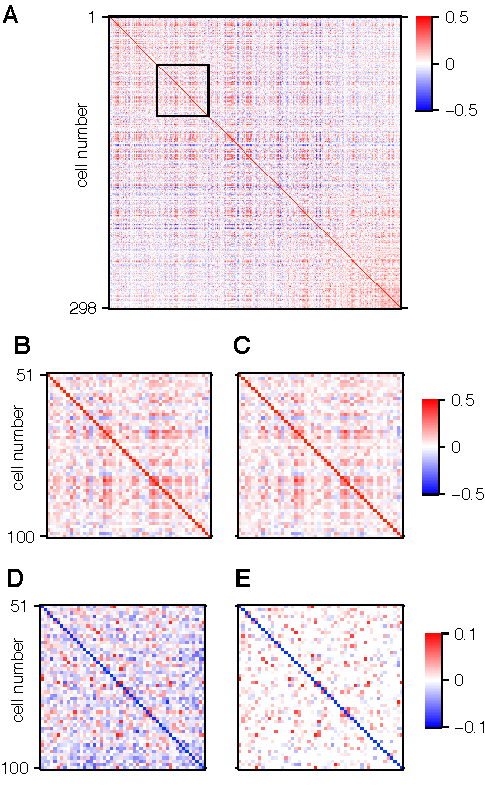
\includegraphics[width=8.3cm]{./figures/Figure01.pdf}}
\end{figure}
\paragraph{Model selection}
Covariance selection is but one of many conceivable low-dimensional approximations of the covariance matrix. Indeed any probabilistic model of the joint population activity regularized toward a small number of parameters automatically defines a low-dimensional approximation of the covariance matrix. Models that accurately reflect the dominant regularities in the activity of the circuit, its so-called `functional connectivity', tend to produce estimates that are nearest to the true value of the covariance matrix and are said to be more \emph{efficient} or to \emph{dominate} other estimators. An estimator's superior efficiency can be ascertained by cross-validation.  Because different types of neural circuits have different types of regularities in their activity, different probabilistic models and covariance matrix estimators may dominate in each case. The estimator that is shown to dominate all others for a specific type of neural circuit may provide the best descriptor of the low-dimensional representation of the correlation structure of the system of interest. Its structure may then be analyzed and related to the circuit's anatomical organization.  
\paragraph{Summary of findings}
In this study, we compared four regularized covariance matrix estimators biased toward different respective low-dimensional correlation structures: `shrinkage toward diagonal' or $C_{\sf diag}$, `shrinkage toward a multifactor model' or $C_{\sf factor}$, `sparse partial correlations' or $C_{\sf sparse}$, and `sparse partial correlations with latent units' or $C_{\sf sparse+latent}$.  First, we demonstrated that, in simulations with known true low-dimensional correlation structures, regularized estimators with matching types of low-dimensional structure generally dominated over the other estimators. We then used cross-validation to determine the most efficient estimator for the population activity of dense groups of neurons in mouse primary visual cortex. We found that $C_{\sf sparse+latent}$ consistently dominated the other estimators.  Estimate produced by $C_{\sf sparse+latent}$ revealed networks of interactions that differed substantially from networks of strongest correlations and depended strongly on the physical distance separating pairs of cells and on the differences in their preferred orientations.

\section*{Results}
% Results and Discussion can be combined.
\paragraph{Covariance estimation}
We considered four regularized estimators based on distinct families of low-dimensional target estimates: `independent', `latent factors', `sparse interactions', and `sparse+latent' (\figref{02}{row 1}).  

\begin{FPfigure}
    \begin{center}
        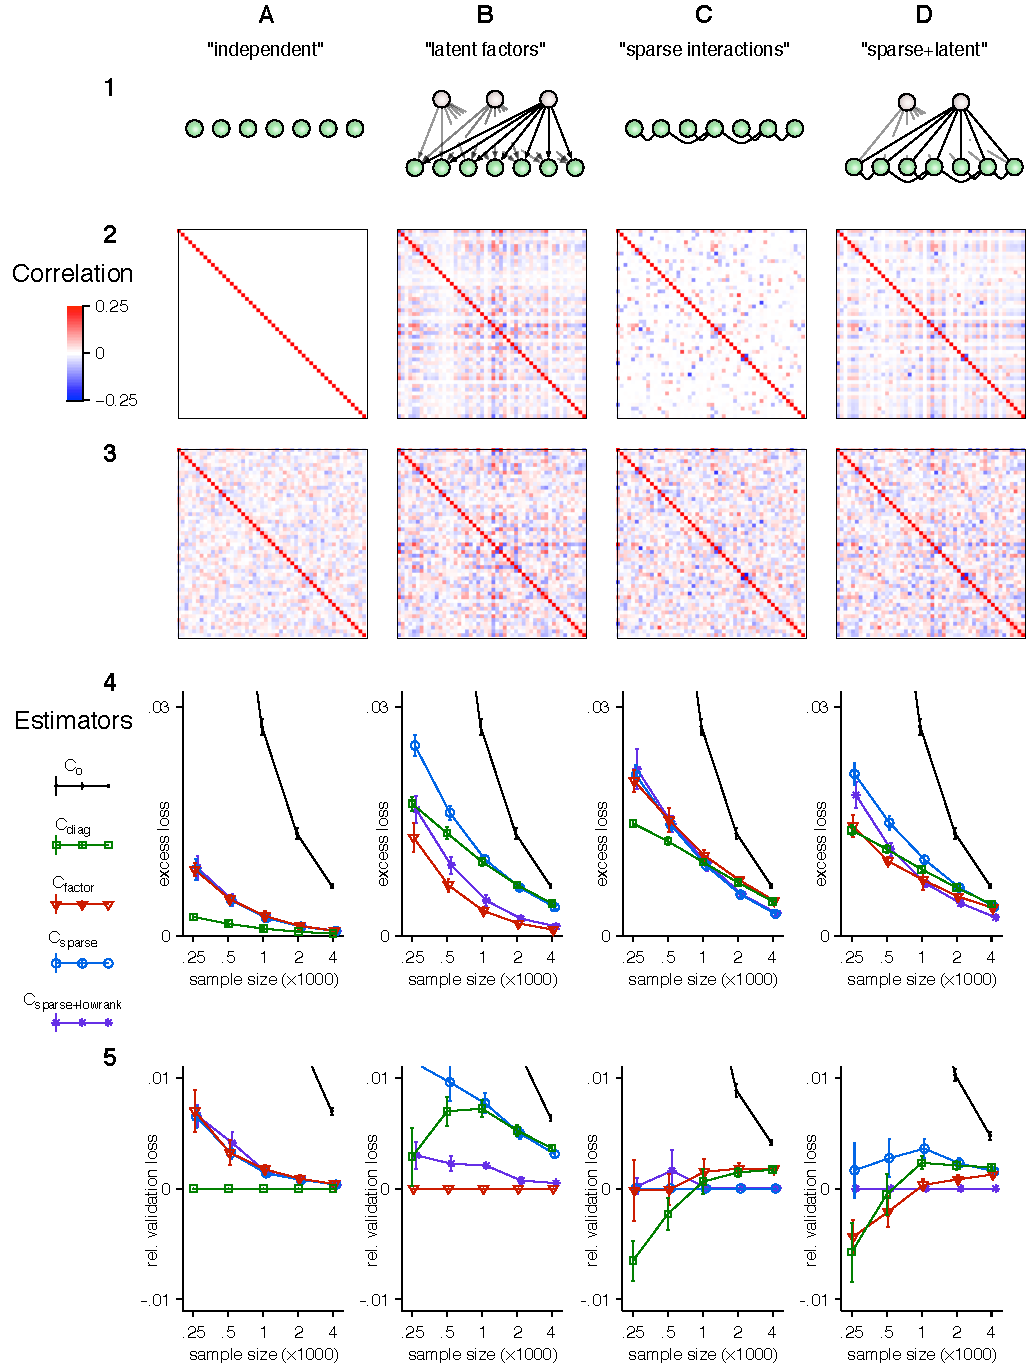
\includegraphics{./figures/Figure02.pdf}
    \end{center}
    \caption{{\bf Estimators whose low-dimensional regularization targets can represent the structure of the true covariance matrix outperform other estimators.}
        {\bf Row 1.} Graphical representations of four types of low-dimensional structures of interactions between observed neurons (green spheres) and latent units (light-shaded spheres).
        In the `independent model' ({\bf A}), observed neurons exert no linear effects on one another neither directly nor through interactions with common latent units. 
        In `latent factors' ({\bf B}), the correlated activity of observed cells is driven by several latent units. 
        In `sparse interactions' ({\bf C}), the correlation matrix is defined by a set of linear interactions between observed neurons. 
        In `sparse+latent' ({\bf D}), correlations arise through direct linear interactions in a sparse subset of observed neurons and through interactions with common latent units. 
        {\bf Row 2.} Examples of $50\times 50$ correlation matrices corresponding to each type of low-dimensional structure. 
        The factor model ({\bf B}) has three latent units. 
        The partial correlation matrix of the sparse model ({\bf C}) is 73\% sparse.
        The `sparse+latent' matrix has one latent unit and its direct interactions are 78\% sparse.
        {\bf Row 3.} Examples of sample correlation matrices calculated from samples of 1000 observations taken from simulated random processes with corresponding correlation matrices from row 2.
        {\bf Row 4.} Mean \emph{excess loss} (Eq.~\ref{eq:excess-loss}) attained by each of the five estimators as a function of sample size. The error bars indicate the standard error of the mean based on 30 samples.
        {\bf Row 5.} Mean \emph{cross-validation loss} (Eq.~\ref{eq:rel-cv-loss}) of covariance estimators with respect to the matching estimator. The values are relative to the validation loss of the estimator that matches the low-dimensional structure of the true covariance matrix. Error bars indicate the standard error of the mean based on 30 samples.
    }
    \label{fig:02}
\end{FPfigure} 

For the first regularized estimator $C_{\sf diag}$, the target estimate is the diagonal matrix $D$ whose diagonal contains  variance estimates. Regularization is achieved by linear \emph{shrinkage} of the unbiased estimate $C_{\sf 0}$ toward $D$ controlled by the scalar \emph{shrinkage intensity} parameter $\lambda \in [0, 1]$:
\begin{equation}\label{eq:c-diag}
C_{\sf diag} = (1-\lambda) C_{\sf 0} + \lambda D
\end{equation}
The diagonal target has structure corresponding to the absence of linear associations between the activity of observed neurons (\figref{02}{A}).  If this structure accurately describes recorded data, then strong shrinkage toward $D$ adds little bias while strongly reducing the variability of the estimate. Shrinkage allows for partial commitment to the low-dimensional representation.  

The target of the second regularized estimator $C_{\sf factor}$, is the factor model $LL^\T + \Psi$, where $L$ is the $p\times d$ matrix of \emph{factor loadings}, where $d$ is the number of factors, and $\Psi$ is the diagonal matrix of independent variances. The estimator, 
\begin{equation}\label{eq:c-factor}
C_{\sf factor} = (1-\lambda) C_{\sf 0} + \lambda (LL^\T + \Psi),
\end{equation}
has two hyperparameters: the number of factors $d$ and shrinkage intensity $\lambda$. The target estimate $LL^\T + \Psi$ has the structure that arises when correlated fluctuations in population activity are linearly driven by a small number of latent factors that affect many cells while direct interactions between cells are insignificant (\figref{02}{B}).   

The third estimator $C_{\sf sparse}$ is based on the assumption that all correlations result from direct linear associations between a sparse set of pairs of observed cells (\figref{02}{C}).  This assumption is enforced by setting to zero an optimal subset of the off-diagonal elements of the precision matrix.  Therefore, $C_{\sf sparse}$ is biased towards correlation structures that arise in networks of linearly interacting pairs of neurons (\figref{02}{C}). The estimator takes the form
\begin{equation}\label{eq:c-sparse}
C_{\sf sparse} = S^{-1},
\end{equation}
where $S$ is a sparse matrix with a large fraction of zeros off the diagonal. The estimate has one hyperparameter that determines the sparsity (fraction of off-diagonal zeros) of $S$.

The fourth estimator $C_{\sf sparse+latent}$, combines the assumptions of the previous two.  The underlying structure arises from sparse interactions between the recorded neurons and latent factors driving their activity (\figref{02}{D}). The estimator has the form \cite{Chandrasekaran:2010,Ma:2013}:
\begin{equation}\label{eq:c-sl}
C_{\sf sparse+latent} = (S - LL^\T)^{-1}
\end{equation}
where, as above, $S$ is a sparse matrix and $L$ is a $d\times p$ matrix of factor loadings. The estimator has two hyperparameters: the number of latent units $d$ and the sparsity of $S$.

\paragraph{Simulation}
To illustrate the performance of the four regularized estimators, we constructed four model populations of $p=50$~neurons each with each matching the correlation structures of a different target estimate (\figref{02}{\,Row 2}).  Sample correlation matrices calculated from samples of size $n=1000$ contain substantial sampling noise (\figref{02}{\,Row 3}) that makes the correlation structure less obvious.

To evaluate the performance of a covariance matrix estimator $C$, we define a real-valued \emph{loss function} $\loss{C,\Sigma}$ that attains a minimum when $C=\Sigma$.  The loss function quantifies the error of the estimate, \emph{i.e.}~the deviation of the estimate $C$ from truth $\Sigma$.

In this study, we adopted \emph{negative normal log-likelihood loss} defined as
\begin{equation}\label{eq:loss}
    \loss{C,\Sigma} = \frac 1 p\left[\ln \det C + \Tr(C^{-1}\Sigma)\right]
\end{equation}
The loss function $\loss{C,\Sigma}$ is related to the multivariate log-likelihood function $L(\Sigma|C_{\sf 0})$ as
\begin{equation}
    L(\Sigma|C_{\sf 0}) = -\frac p 2 \ln(2\pi) -\frac p 2 \loss{\Sigma,C_{\sf 0}}
\end{equation}

We normalized the loss function by $\frac 1 p$ to make its value comparable across different population sizes. 

The choice of loss function is motivated by mathematical convenience. We expect that the main conclusions of our study will not change qualitatively with other well behaved loss functions, such as the Frobenius norm of the difference $\|C-\Sigma\|_F$ \cite{Ledoit:2004,Schafer:2005}, Stein's entropy loss, or quadratic loss \cite{James:1961,Fan:2008}.  

We define the \emph{excess loss} as
\begin{equation}\label{eq:excess-loss}
    \eloss{C,\Sigma} = \loss{C,\Sigma}-\loss{\Sigma,\Sigma},
\end{equation}
which assumes zero at its minimum. 

In Figure \ref{fig:02}, row 4 shows the mean excess losses and their standard errors calculated from 30 samples of sizes n=250, 500, 1000, 2000, and 4000 for each estimator and each ground truth. For each estimator, hyperparameters were estimated by nested cross-validation (See Methods for more details.)

As expected, estimators with whose structure matched that of the true model typically outperformed the other estimators. There were two exceptions: First, for small sample sizes, there was insufficient data to reveal the true correlation structure. In this case estimates with simpler targets often outperformed the estimator based on the correct model. Second, the sparse+latent estimator often performed equally well to the sparse estimator even when the data did not have any latent units.  In these cases, it inferred the right number of latent units: zero. In larger models, the falsely identified latent factors are more common.

When the ground truth, $\Sigma,$ is not accessible, loss can be estimated solely from the data through \emph{validation}.  In validation, an additional independent \emph{testing sample} is used to compute a sample covariance estimate $C_{\sf 0}^\prime$.  Then \emph{validation loss} $\loss{C,C_{\sf 0}^\prime}$ can be used as an unbiased estimate\footnote
{
    Validation loss $\loss{C,C_{\sf 0}^\prime}$ is an unbiased estimate of loss $\loss{C,\Sigma}$ when $\loss{\cdot,\cdot}$ is \emph{additive} in its second argument so that 
 \begin{equation*}\label{eq:additivity}
 \loss{C,z_1} + \loss{C,z_2} \equiv \loss{C,z_1+z_2}
 \end{equation*}

Then the absence of bias can be shown:
\begin{equation*}
    \E{\loss{C,C_{\sf 0}^\prime}}=\loss{C,\E{C_{\sf 0}^\prime}}=\loss{C,\Sigma}
\end{equation*}

This property does not hold for some other popular loss functions such as Stein's entropy loss, for example, which prevents their substitution with corresponding validation losses. However, various other loss functions do have this property and could have been used.
} 
of loss $\loss{C,\Sigma}$.  Thus, estimators resulting in consistently lower validation loss can be inferred to produce estimates that are closer to truth than estimators with higher validation loss. 

With empirical data, acquiring a separate testing sample is not practical. Instead, $K$-fold cross-validation is used: The sample is divided into $K$ subsets of approximately equal size ($K=10$ in this study).  Then each subset is used as the validation sample with the other $K-1$ serving as a training dataset. The validation losses from each of such `folds' are averaged to produce \emph{cross-validation loss} or \emph{CV-loss} for short.  Let $C_{\sf 0}^{\{k\}}$ denote the sample covariance matrix computed from the $k^{th}$ subset and $C^{\{\setminus k\}}$ denote the results of estimator $C$ trained on the remaining $K-1$ subsets. Then cross-validation loss for estimator $C$ is
\begin{equation}\label{eq:cv-loss}
    \ell_C=\frac 1 K \sum\limits_{k=1}^K \loss{C^{\{\setminus k\}},C_{\sf 0}^{\{k\}}}
\end{equation}
In the present formulation, $\ell_C$ is known as the cross-validated Gaussian log-likelihood (up to a constant offset and multiplier).

Since we only need to compare estimators to each other, we are only interested in \emph{relative} CV-loss of estimator $C$ with respect to reference estimator $C_{\sf ref}$:
\begin{equation}\label{eq:rel-cv-loss}
    \ell_{C,C_{\sf ref}} = \frac 1 K \sum\limits_{k=1}^K \left[
        \loss{C^{\{\setminus k\}},C_{\sf 0}^{\{k\}}} -
    \loss{C_{\sf ref}^{\{\setminus k\}},C_{\sf 0}^{\{k\}}} 
\right]
\end{equation}

In simulation, CV-loss accurately reproduced the differences between the estimators' excess losses, although with greater variability (Figure \ref{fig:02}, Row 5). For each kind of ground truth (Row 2), relative CV-losses were computed with respect to the estimator whose regularization target matched the structure of the respective ground truth. Just as with excess loss in Row 4, the means and their standard errors were computed from 30 samples taken for each ground truth and for each sample size.

These simulations demonstrate that with sufficiently large sample sizes the most efficient among several regularized estimators could be used to infer the most likely type of low-dimensional structure present in the data.

\paragraph{Covariance estimation in neural data}
We recorded calcium activity in dense populations of neurons in the supragranular layers in primary visual cortex of anesthetized mice using fast random-access 3D scanning two-photon microscopy \cite{Reddy:2005, Katona:2012, Cotton:2013}. We presented 300 repetitions of full-field drifting gratings with two directions of motion or 150 repetitions with five directions (\figref{03}{A}) on one side of the visual field of anesthetized mice. Groups of cells loaded with a calcium-sensitive fluorescent dye were imaged and localized in 3D space (\figref{03}{B and E} in the visual cortex on the contralateral side to the stimulus. Using acousto-optic deflectors (AOD) to steer the laser in 3D,  we recorded the somatic calcium activity from the located cells with concurrent motion detection \cite{Cotton:2013}.  This technique allowed fast sampling (100--150 Hz) from large numbers (150--350) of cells in a small volume of cortical tissue ($200\times200\times100$ $\mu$m$^3$) in layers 2/3 and 4 (\figref{03}{C}). After downsampling the signal to 20 Hz, relative firing rates were inferred using sparse nonnegative deconvolution \cite{Vogelstein:2010} (\figref{03}{C and D}). Only cells that produced detectable calcium activity were included in the analysis (See Methods). The average stimulus response was subtracted from each trial; the remaining signals were further downsampled into 150 ms bins to compute the noise correlation matrix (\figref{ 03}{F and G}). The durations of recordings dedicated to estimating the noise correlations ranged between 15--20 minutes.  Besides the high-repetition stimulus protocol used to estimate noise correlations, an orientation tuning stimulus protocol was used to map the orientation tuning of each cell (\figref{03}{E}). Overall, 31 imaged sites from 24 animals were included in the study.

\begin{figure}    \floatbox[{\capbeside\thisfloatsetup{capbesideposition={right,center},capbesidewidth=8.3cm}}]{figure}[\FBwidth]
    {\caption{{\bf Acquisition of neural signals for the estimation of noise correlations.}
    Visual stimuli comprising full-field drifting gratings interleaved with blank screens ({\bf A}) were presented to anesthetized mice while two-photon recordings of somatic calcium signals were collected using fast 3D random-access microscopy ({\bf B}). The visual stimulus included an initial period with 16 directions of motion for orientation tuning followed by a longer (15--20 min) period of stimulation with only 2 or 5 directions of motion for the computation of the noise correlation matrix. 
    {\bf C.} Representative calcium signals from eight cells out of 298 cells downsampled to 20 Hz. The inferred firing rate binned in 150 ms intervals are indicated by red ticks below each trace.
    {\bf D.} The raster plot of the inferred firing rates, binned in 150 ms intervals, from the entire population from the first (left) and last (right) minute of the entire recording.  The traces from {\bf C} are highlighted in red.
    {\bf E.} The spatial arrangement and orientation tuning of the 298 cells from the imaged site.
    {\bf F.} The noise correlation matrix of the activity of the neural population. 
    {\bf G.} Histogram of noise correlation coefficients. The red line indicates the mean.
} \label{fig:03}}
    {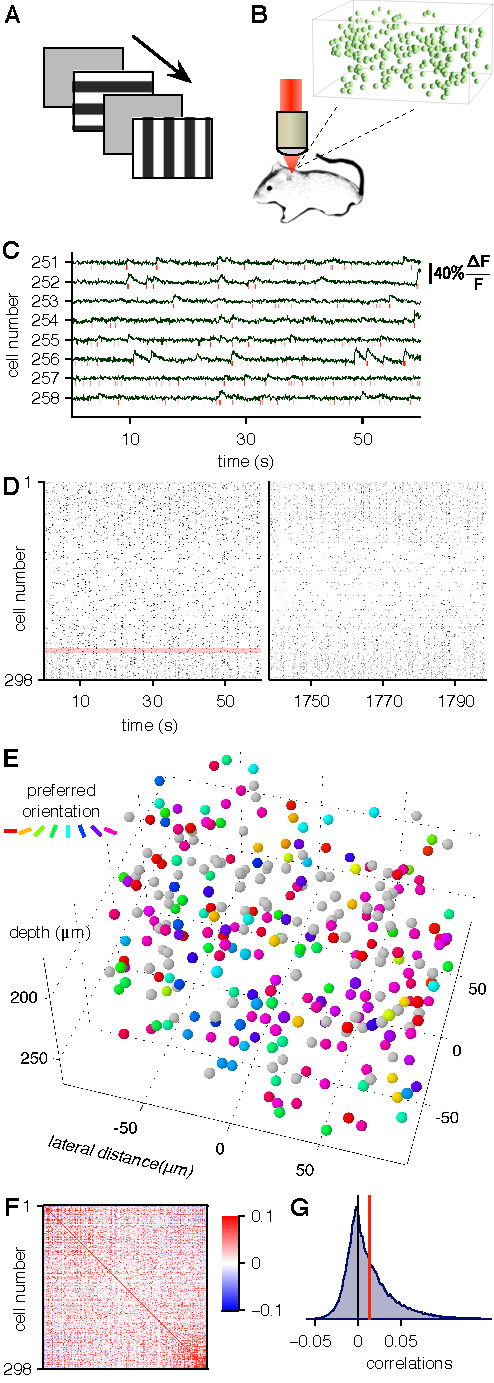
\includegraphics[width=8.3cm]{figures/Figure03.pdf}}
\end{figure}

In these highly localized populations both direct interactions between cells and common diffuse inputs likely contribute to overall population co-variability.  We therefore hypothesized that regularized estimates capturing a sparse partial correlation structure, and/or interactions with latent units would be the most efficient. At the same time, average correlations were relatively small (\figref{03}{G}), giving a potential advantage to estimates biased toward independence (\emph{e.g.}\;$C_{\sf diag}$). Finally, correlation structure could possibly be best explained by common fluctuations across the entire population, to the advantage of estimates biased toward low-rank correlation structure (\emph{e.g.}\;$C_{\sf factor}$, $C_{\sf factor+lowrank}$). Thus it was \emph{a priori} unclear which estimator would perform best.

We found that estimator $C_{\sf sparse+latent}$ was the most efficient (Fig.~\ref{fig:04}). The median relative CV-validation loss (Eq.~\ref{eq:rel-cv-loss}) of each of the estimates $C_{\sf 0}$, $C_{\sf diag}$, $C_{\sf factor}$, and $C_{\sf sparse}$ with respect to $C_{\sf sparse+latent}$ was significantly above zero ($p<0.001$, Wilcoxon signed rank test, for each).

\begin{figure}[!ht]    \floatbox[{\capbeside\thisfloatsetup{capbesideposition={right,center},capbesidewidth=8.3cm}}]{figure}[\FBwidth]
    {\caption{{\bf The sparse+latent estimator $C_{\sf sparse+latent}$ outperforms the other estimators on neural data.}
    {\bf A--D.} Histograms of average cross-validation loss differences of the respective estimators $C_{\sf 0}$, $C_{\sf diag}$, $C_{\sf factor}$, and $C_{\sf sparse}$ from $C_{\sf sparse+latent}$. 
    The histograms are based on 31 imaged sites in 24 mice. 
    All medians (red dashed lines) were significantly greater than zero, indicating the dominance of $C_{\sf sparse+latent}$ over the other estimators. 
    The green arrows indicate the results for the site shown in Fig.~\ref{fig:03} and Fig.~\ref{fig:05}
    } \label{fig:04}}
    {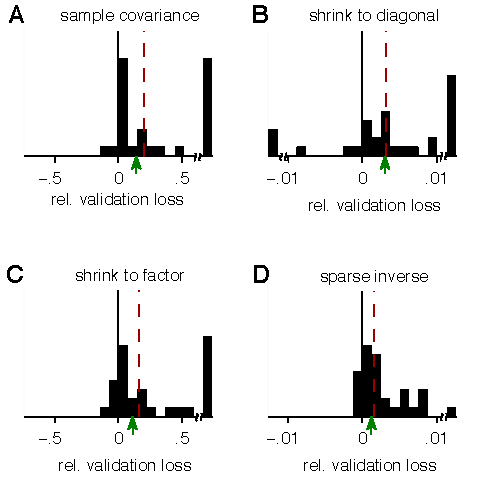
\includegraphics{./figures/Figure04.pdf}}
\end{figure}

\paragraph{Correlation structure and circuit architecture}
Having demonstrated that $C_{\sf sparse+latent}$ dominated the other estimators, we examined the low-dimensional structure revealed by this estimator for individual imaged sites. By design, the sparse+latent estimator finds the optimal balance between a sparse network of partial correlations and shared common latent units. If this estimate dominates, we can hypothesize that it is better reveals underlying physiological interactions than the usual correlations. In particular, the sparse component of the partial correlation matrix suggests direct interactions between pairs of neurons, whereas the low-rank component suggest common fluctuations such as those caused by common inputs or other collective synchronized activity. 

We examined the structure of the sparse+latent estimate at individual sites (an example site is depicted in Fig.\;\ref{fig:03}). At these sites the regularized estimate of the correlation matrix appeared very similar to the unregularized sample correlation matrix (Fig.~\ref{fig:05}\,A and D). However, the corresponding partial correlation matrices differed dramatically (Fig.~\ref{fig:05}\,B and E). The partial correlation was decomposed into sparse and low-rank components (Fig.\,\ref{fig:05}\,C). Although correlations were mostly positive, the sparse partial correlations (or `interactions'), had a much larger fraction of negative values than sample correlations. The sparse component had 82.1\% sparsity (or 17.9\% connectivity), which corresponded to the average node degree (interactions per cell) of 52.5 (Fig.\;\ref{fig:05}\,G). The low-rank component had rank 17.

\begin{FPfigure}
    \begin{center}
        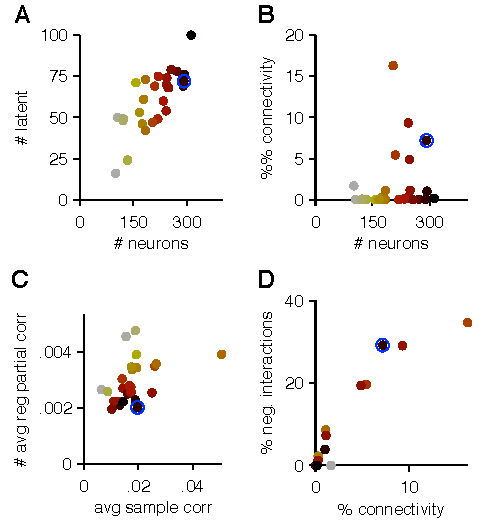
\includegraphics[width=17.35cm]{./figures/Figure05.pdf}
    \end{center}
    \caption{{\bf Example of low-dimensional correlation structure revealed by the sparse+low-rank estimator.}
    {\bf A.} The regularized estimate of the correlation matrix (top-right) closely approximates the sample correlation matrix (bottom left). 
    This close approximation is  also demonstrated by the scatter plot of the correlation coefficients produced by the two estimates ({\bf D}). 
    However, the partial correlation matrices from the two estimate show more pronounced differences ({\bf B} and {\bf E}). 
    {\bf C.} Furthermore, the partial correlation matrix of the regularized estimate is decomposed into a sparse component with 82.2\% off-diagonal zeros (bottom-left) and low-rank component of rank 15 (top-right).
    {\bf F.} The sparse component of the regularized partial correlation matrix had little resemblance to the sample correlations. The gray interval indicates the range of correlations containing 82.2\% of cells pairs, equal to the fraction of zeros in the sparse partial correlation matrix. This interval contained 58.9\% of the partial correlations. 
    {\bf G.} The graphical depiction of the positive (green) and negative (magenta) partial correlations as edges between observed neurons. The line density is proportional to the magnitude of the correlation.
    {\bf H.} A subset of neurons from the center of the cluster shown in {\bf G} showing the regularized partial correlations.
    {\bf I.} The same subset with sample correlations thresholded to match the sparsity of the regularized interactions.
}
\label{fig:05}
\end{FPfigure}

In previous studies of the structure of correlations, a sparse network was produced by thresholding the correlations coefficients at a level deemed significant. A network was formed by connecting neurons whose total correlations exceed this threshold \cite{Golshani:2009,Malmersjo:2013}. There was fairly little overlap between the network of interactions revealed by such thresholding and those revealed by the sparse+latent estimator (\figref{05}{F}). When thresholded to the same sparsity (82.1\%), only 42\% of cell pairs connected in one network were connected in the other while the average magnitude of such correlations was much lower in the case of the regularized estimator (\figref{05}{F, H, and I}). In particular, many low sample correlations translated into negative interactions in the regularized estimate. Indeed, the absence of correlations between pairs of cells that both correlate similarly to several of their neighbors should be considered as significant as a high correlation coefficient. Regularized partial correlations reveal such phenomena whereas regular sample correlations cannot.

The average partial correlations revealed by the sparse+latent estimator at all 31 sites were about 5 times lower than the sample correlations and  less variable across sites (\figref{06}{A}). The average node degree of the sparse component of the partial correlations and the number of inferred latent units varied widely between sites but generally increased with recorded population size (\figref{06}{B and C}). However, there was an inverse relationship between the number of latent units and the average node degree (\figref{fig:06}{D}). Several sites, even with relatively large population sizes, had fairly few pairwise interactions and were dominated by latent units.  These differences have multiple explanations, including differences in brain states and recording quality (neuropil contamination, motion). 

\begin{figure}[!ht]
    \begin{center}
        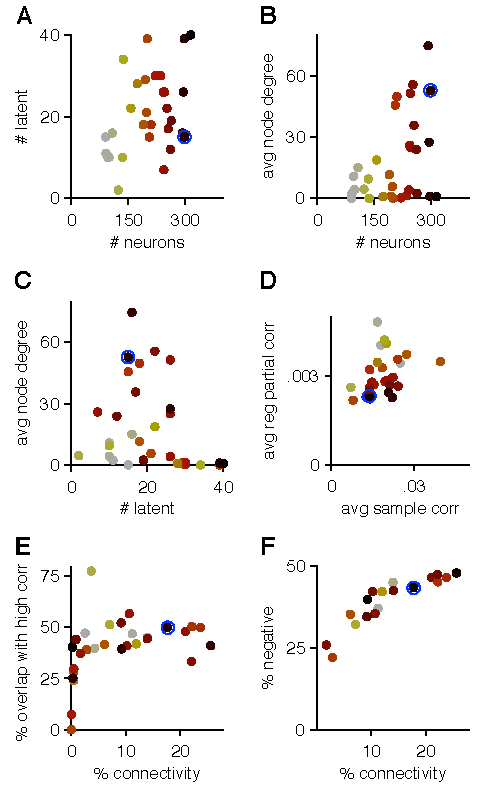
\includegraphics{./figures/Figure06.pdf}
    \end{center}
    \caption{{\bf Properties of sparse+low-rank regularized estimates from all imaged sites}
    {\bf A.} The average sample correlations vs.~average partial correlations for each imaged site. In each plot, the red asterisk indicates the site shown in figures \ref{fig:03} and \ref{fig:05}.
    {\bf B.} The average node degree for sparse partial correlations vs.~population size in each imaged site. 
    {\bf C.} The number of inferred latent units vs.~population size in each imaged site.
    {\bf D.} The number latent units vs.~average node degree for sparse partial correlations for each site.
}
\label{fig:06}
\end{figure}

We also examined the relationship of differences in orientation preference and physical distances (lateral and by depth) between pairs of cells to the average sample correlations, average regularized partial correlations, and inferred connectivity between them (Fig.\;\ref{fig:07}). The average partial correlations fell more rapidly with difference in preferred orientation (\figref{fig:07}{A and D}) and lateral displacements at equal depths ($\pm 25\;\mu$m) (\figref{07}{B and E}), and differences in depth at small ($\pm 25\;\mu$m) lateral displacements (\figref{07}{C and F}).

\begin{figure}[!ht]
    \begin{center}
        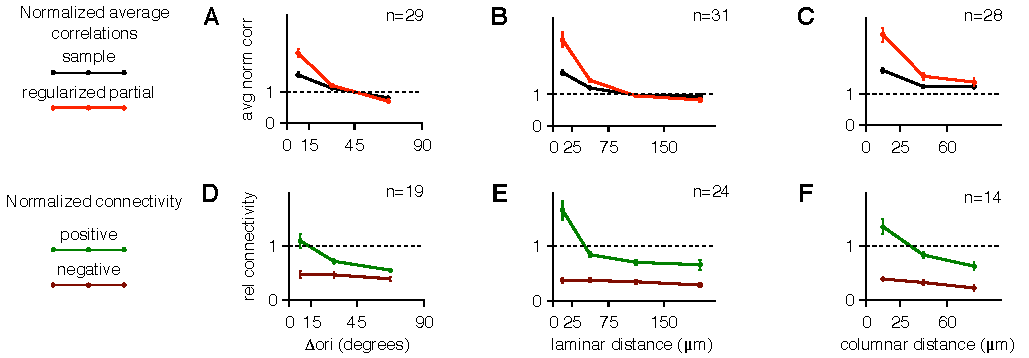
\includegraphics{./figures/Figure07.pdf}
    \end{center}
    \caption{{\bf Dependence of correlations and partial correlations on orientation tuning differences and physical distance between cell pairs.}
    {\bf A--C.} Average partial correlations (red) estimated by $C_{\sf sparse+latent}$ and average sample correlations (black) averaged across multiple imaged sites. In each site, the correlations were normalized by the respective average correlation shown in Fig.\;\ref{fig:06}\,A.  The number $n$ of sites that qualified to be included in the analysis is indicated. Sites were included if they had at least 20 pairs of neurons in each of the intervals. The error bars indicate the standard error of the mean for based on $n$.
    {\bf A.} Average correlations between pairs of neurons tuned to orientation with differences in preferred orientation in the intervals of 0--15$^\circ$, 15--45$^\circ$ and 45--90$^\circ$. 
    {\bf B.} Average correlations between pairs of neurons located at the same depth ($\pm$25$\mu$m) separated by lateral distances in the intervals of 0--25 $\mu$m, 25--75 $\mu$m, 75--150 $\mu$m, and 150+ $\mu$m.
    {\bf C.} Average correlations between pairs of neurons displaced laterally by less than 25 $\mu$m separated in depth by distances in the intervals of 0-25 $\mu$m, 25--60 $\mu$m, and 60+ $\mu$m.
    {\bf D--F.} Normalized connectivity of positive (green) and negative (dark red) interactions from the sparse component obtained from $C_{\sf sparse+latent}$. Normalized connectivity was computed as the fraction of pairs connected by interactions of corresponding signs in each interval divided by the fraction of non-zero interactions across the entire site. Site were included in the analysis only if they had at least 20 cell pairs in each interval. The error bars indicate the standard error of the mean based on the number $n$ of sites included in the analysis.
}
\label{fig:07}
\end{figure}

The connectivity expressed by the partial correlations in the regularized estimate had different organization for positive and negative interactions. Positive interactions fell rapidly as a function of difference in preferred orientation (\figref{07}{D}), lateral displacements (\figref{07}{E}), and displacement in depth (\figref{07}{F}). Negative interactions were much less selective (\figref{07}{D--F}).

\section*{Discussion}
\paragraph{Functional and anatomical connectivity}
Systems neuroscience is the quest to discover principles whereby anatomical organization of neural circuits gives rise to their function.  This line of inquiry requires expressive descriptions of the observed activity of neural circuits. 

The term \emph{functional architecture} most commonly refers to stimulus response properties of neurons \cite{Reid:2012}. Over the past 50 years, tremendous progress has been made in relating the functional architecture to the anatomical, synaptic wiring of neuronal populations and individual neurons.  This line of inquiry is based on the view of the brain as a complex filter of external stimuli. 

In contrast to functional architecture, \emph{functional connectivity} commonly refers to the degree of correlation, synchronization, or other forms of statistical association between neuronal populations or individual neurons inferred from spontaneous activity or trial-to-trial variations,  not directly driven by external stimuli.  Functional connectivity is thought to reflect internal, recurrent connectivity in neural circuits.  This line of inquiry ascribes greater significance to the brain's intrinsic activity (often dismissed as `noise') \cite{Yuste:2005}. However, relatively little progress has been made in understanding the role of functional connectivity and its relationship to the anatomical connectivity.

Neural correlations boast a rich history as indicators of functional connectivity. When measured on temporal scales of milliseconds, sharp peaks or troughs in the cross-correlogram between pairs of neurons at latencies typical of synaptic transmission provide evidence of monosynaptic connection between pairs of cells \cite{Moore:1970,Alonso:1998,Denman:2013} (although other processes can also generate sharp peaks in the cross-correlogram while many synaptic connections may not produce such signatures). Without targeted stimulation of specific cells or measurements of subthreshold intracellular events, such analysis remains the best method for detecting probable monosynaptic connections in vivo. When measured at longer temporal scales, neural correlations reflect activations involving large ensembles of neurons and may reflect direct causal anatomical interactions, indirect causal interactions, or complex network-wide emergent features of activity with little correspondence to the local anatomical connectivity. These slower correlations correspond more closely to the computation performed by the circuit than to its anatomical organization. For this reason, firing rate correlations at scales of tens to hundreds milliseconds have been studied for their effect on coding under the assumption of rate codes and linear downstream decoder \cite{Averbeck:2006} with little interest in anatomy.  Calcium imaging allows simultaneous measurements of the activity of large populations of cells \emph{in vivo} \cite{Katona:2012,Cotton:2013} and even of entire nervous systems \cite{Leung:2013,Ahrens:2013}, but its temporal bandwidth is limited to the scale of tens or hundreds milliseconds by the kinetics of calcium-sensitive dyes, limiting its use to slower temporal scales at which correspondence between functional and anatomical connectivity is less direct.

Our study is part of the effort to find descriptions of functional connectivity with the greatest chance of correspondence to anatomical, causal organization of the circuit.

\paragraph{Extraction of the correlation structure}
The word `structure' implies a succinct, simplified representation that captures only the essential, significant features. Several forms of correlations structure can be extracted from the same data and used to describe functional connectivity in different ways.

Perhaps the least sophisticated yet common approach for extracting the structure of correlations is to threshold above a selected level of significance. Part of the appeal of thresholded correlations is their representation in the form of graphs that can be related to graphs of synaptic connectivity and made amenable to network analysis \cite{Bullmore:2012}. For example, \cite{Malmersjo:2013} analyzed the graph theoretical properties of networks of thresholded correlations in development. 

Alternatively, the correlation structure may be extracted in the form of low-rank approximations computed by principal component analysis, factor analysis, or activation maps conditioned on the activity of a single neuron. Low-rank components show synchronous multineuronal activation patterns without revealing graphs of interactions between neurons. They are often interpreted as emergent patterns of large circuits or brain state fluctuations \cite{Kenet:2003}.

Another reduced representation of correlation matrices is obtained by sparsifying its inverse, resulting in a graph of partial correlations. Under the assumption of a multivariate normal distribution or, more generally, an elliptical distribution, sparse partial correlations suggest a sparse network of dependencies, \emph{i.e.}\;a probabilistic graphical model. This property has led some investigators to propose that sparse inverse approximation of correlations may serve as closer estimates of direct anatomical interactions between brain regions in imaging studies than correlations \cite{Varoquaux:2012,Ryali:2012}. However, since deviations from elliptical distribution disrupt the correspondence between partial correlations and linear dependencies \cite{Loh:2012}, it is not clear whether this is indeed  the case. Partial correlations are meaningful when most interacting variables are observed. Perhaps for this reason, until now, partial correlations had not been considered in analysis of multineuronal recordings.

In this study, we sought to uncover the optimal low-dimensional approximation of the covariance matrix for efficient estimation of the true covariance matrices in cortical microcircuits on the temporal scale of 100--200 ms corresponding to the temporal resolution of spike rates from somatic calcium signals \cite{Cotton:2013}.  We found that networks of partial correlations were more statistically efficient than low-rank approximations of correlation matrices (Fig.\;S\ref{supp:01}\;E). Furthermore, estimation became still more efficient when low-rank components were allowed to be combined with sparse partial correlations. We propose that correlation structures that are supported by the data  are more likely to reflect anatomical, causal interactions. The network of sparse partial correlations suggests interactions between specific pairs whereas the low-rank represents emergent activity patterns involving collective activations of larger circuits or global fluctuations. The revealed network of partial interactions was substantially different from that revealed by thresholding correlations (\figref{05}{C, F, H, I}). In particular, it shows that many low correlations correspond to strong negative interactions (\figref{05}{F}). Intuitively, this suggests that many low interactions are as surprising or significant considering the common correlations with other neurons. The analysis of sample correlations does not ascribe significance to correlation coefficients that are surprisingly low, based on their common correlations to other cells.


\paragraph{Functional connectivity from probabilistic models}
Increasingly, functional connectivity is inferred by fitting probabilistic models such as various forms of multivariate Gaussian models, linear-nonlinear models, Generalized Linear Models \cite{Pillow:2008}, and maximum entropy models \cite{Schneidman:2006, Tkacik:2006, Tang:2008, Shlens:2009}. In probabilistic models, functional dependencies are defined by multiplicative terms comprising the model. If the model can be decomposed as a product of terms so that a pair of variables can be segregated into separate terms, the two variables are conditionally independent: the activity of one neuron can be predicted from other neurons just as well with or without considering the second neuron, suggesting a lack of a direct causal interaction between them. Probabilistic models allow inferring latent variables to account for the activity of unobserved circuitry.


\paragraph{Model selection}
Various estimation methods infer very different structures of functional connectivity from the same data. What kind of structure expresses most relevant information? How does one determine which functional connectivity structure is best supported by the empirical data? The field of machine learning offers a rich toolbox of model selection criteria. Parametric criteria such as the \emph{Bayesian model selection criterion}, \emph{Akaike Information criterion}, and \emph{Bayes (or Schwartz) Information Criterion} (BIC) are computationally efficient but rely on generally unsupportable assumptions about the data generating process.  The most assumption-free yet more computationally intensive are procedures based on cross-validation \cite{Arlot:2010} and, when models have hyperparameters, nested cross-validation to select their values. It is commonly assumed that probabilistic models that demonstrate the highest average cross-validated log likelihood yield a better representation of the functional connectivity. For example, \cite{Ganmor:2011} demonstrated that their proposed Reliable Network Model (a maximum-entropy model on the multivariate binary domain constrained by a sparse heuristically selected network of correlations of several orders) yielded higher cross-validated log-likelihoods than the full-pairwise Ising model. The authors use this fact to support the claim that the former model revealed a more anatomically relevant structure of functional connectivity than the pairwise Ising model.

However, in simulation, we showed that, more constrained, simpler models often outperformed complex models in cross-validation studies even when their structure was differed from the true structure (\figref{02}{row 5}), only because these more constrained models were less sensitive to sampling noise. Therefore, by itself, better cross-validation performance of a model does imply closer correspondence of its structure to the functional structure of the data generating process. For example, a properly sparsified pairwise Ising model could outperform the Reliable Network model.  Unfortunately, optimal sparsification of Ising models is no computationally tractable procedure exists to infer the optimal sparse structure of dependencies in an Ising model.

In our study we selected between families of models based on their cross-validation performance. The winning model family was more flexible than the others and therefore more susceptible to noise. The fact that it still performed better indicated that the additional features were required. We conclude that under these circumstances, the selected model can be asserted to better represent the true structure of the data generating process, at least in comparison to the other three models.

In our study, we focused on estimating a specific parameter of the distribution (its covariance matrix) rather than fitting a specific parametric distribution.  Under the loss function (Eq.~\ref{eq:loss}) we selected, the covariance matrix estimation methods are equivalent to fitting a multivariate Gaussian model and selecting the best structure on the basis of cross-validated log-likelihood. However, the ranking of models was preserved under other loss functions (Fig.~S\ref{fig:supp02}), indicating that model selection results were not strongly dependent on the assumption of gaussianity. We defend the practice of evaluating and optimizing probabilistic models with respect to their parameters that are more relevant for functional connectivity rather than maximizing their cross-validated log likelihoods, which are sensitive to all parameters. For example, model A may attain higher cross-validated log likelihood than model B due to its better ability to capture the tails of the distribution while model B better estimates the correlation matrix. We maintained that model B must be more relevant for studies of functional connectivity because correlations do reflect aspects of functional connectivity.

The correlation structures we considered also corresponded to structures of conditional dependencies in multivariate Gaussian models or, more generally, elliptical distributions. For example, zero partial correlation indicates conditional independence between a pair of variables under an elliptical distribution, but this correspondence weakens or breaks down with deviation from elliptical distributions \cite{Loh:2012}.  Other probabilistic models, when optimally sparsified for best cross-validated estimation of the covariance matrix, could suggest very different forms of low-dimensional representations (structures) of the covariance matrix. For example, spatiotemporal Ising models, marginalized to reproduce the correlation matrix at the same temporal scale, would suggest an alternative correlation structure from the same data. At this time we do not have computationally efficient methods for finding sparse structures of dependencies in Ising models optimized with respect to cross-validated estimation of their cross-correlation matrices. If we did, and the estimator thus constructed outperformed our $C_{\sf sparse+lowrank}$ estimator, we would be adopt this new estimator as one producing the best structure of the connectivity. Various forms of GLMs could also be evaluated with in the same way: sparsified for best estimation of the covariance matrix (not log-likelihood) and compared to the estimators studied in this study.  Again, if this new covariance estimator outperforms, $C_{\sf sparse+lowrank}$, we will be compelled to adapt it for estimating the functional connectivity.

\paragraph{Big neural data}
Transformational breakthroughs in systems neuroscience are anticipated to follow the ongoing technological advances that will allow simultaneous recordings of the spiking activity of much larger subsets of neurons in functioning neural circuits than have been possible thus far \cite{Alivisatos:2013}. It is far from certain whether massively multineuronal recordings will readily reveal new principles of neural function by application of current statistical techniques. Large datasets aggravate the numerical problems and the model selection caveats described in this paper. The number of parameters in models of population activity grows quadratically.  Models of joint population activity feature large numbers of parameters, that growing quadratically or faster with population size. Without ways to restrict such models, they quickly become ill conditioned (e.g. \cite{Roudi:2009}.  Statistical models of population activity will need to have both correct mathematical forms of interactions and optimal ways of restricting them so that the total number of estimated parameters remains commensurate with the amount of measurements. 

Our study employs regularization, which restricts the models based on the data itself. Other models may use restrictions that are based on various heuristics in addition to regularization.  These methods have numerous caveats when it comes to inferring the optimal structure of functional connectivity from such methods. Improved estimation of covariances and the general framework of producing such estimators for specific neural populations can be applied to various circuits and serve as a statistical description of their functional organization. 

\paragraph{Correspondence to anatomical organization}
If the ultimate goal of this line of inquiry to find descriptions of functional connectivity that are most informative about the anatomical and physiological organization of the circuit, then the models must be directly validated according to their correspondence to the anatomical organization. Little empirical evidence presently exists to show which models of connectivity, when fitted to the recordings of activity, reveal functional connectivity with best correspondence to anatomical connectivity. 

In this study we find that the structure of partial correlation of the optimal estimator had stronger dependencies on the separation in depth, lateral position, and orientation preferences than sample correlations (\figref{07}{A--C}). The inferred positive and negative partial correlations too had different structures COMPARED TO NOISE CORRELATIONS ?? (\figref{07}{D--F}).  Also the average partial correlations were more consistent between imaged sites than average sample correlations (\figref{06}{A}). Although these effects could conceivably results from trivial numerical artifacts, they are consistent with improved representation of functional connectivity by the proposed estimator.

Additional studies with additional markers of circuit architecture such as cell types and synaptic connectivity could shed additional light on the ability of models to reveal meaningful functional connectivity.  For example, labeled interneurons could be studied for their distinct connectivity patterns contrasted with pyramidal cells. I THIKN WE NEED ONE LAST SENTNECE HERE TO SAY THAT FUNCTIONAL CONNECTIVITY IF IT RELATED TO ANALTOMICAL IS IMPORTANT SINCE IT CAN TELL US HOW CIRCUITS INTERACT TO COMPUTE MENTION EXAMPLE OF STATES, SLEEP HERE ETC. I.E. GROUPS CELLS MAY BE CONNECTED BUT ONLY INTERACTING IN STATE A AND NOT B. 

\section*{Methods}
% You may title this section "Methods" or "Models". 
% "Models" is not a valid title for PLoS ONE authors. However, PLoS ONE
% authors may use "Analysis" 
\paragraph{Data Acquisition}
Fast 3D two-photon imaging of calcium signals \emph{in vivo} was performed as described in \cite{Cotton:2013}

\paragraph{Cross-validation}
To compare the performance of the estimator against each other, we used conventional 10-fold cross validation to measure cross-validation loss (Eq.~\ref{eq:cv-loss}). Briefly, each recording was split into 30 blocks of equal duration.  The 30 blocks were then grouped randomly into 10 datasets with 3 blocks in each.  This procedure ensured sufficient independence between the 10 datasets while still ensuring that each dataset included data from different parts of the recording.   Then, each dataset was used as the testing dataset with the rest of the data used for estimating the covariance matrix.  

Since each of the regularized estimators had one or two hyperparameters, we used \emph{nested cross-validation}.  The outer loop evaluated the performance of the estimators with optimal values of the hyperparameters.  The optimization of the hyperparameters was performed within the inner loop in two phases: random search to find a good starting point and pattern search to find the global minimum.  The inner cross-validation loop subdivided the training dataset from the outer loop to perform 10-fold cross-validation in order to evaluate each choice of the hyperparameter values.  Thus the size of the training dataset within the inner loop comprised 81% of the entire recording.

When cross-validation loss was not required, only the inner loop of cross-validation was used, applied to the entire dataset.  This approach was used to compute the covariance matrix estimates and their excess-loss in the simulation study (\figref{02}{\;rows 3 and 4}) and to analyze the partial correlation structure of the sparse+latent estimator (Fig.~\ref{fig:05}--\ref{fig:07}).
\paragraph{Covariance Estimation}
Within the inner loop of cross-validation, covariance matrix estimation was performed with fixed hyperparameter values provided by the search algorithm.  The computation of each regularized estimator only required the sample covariance matrix $C_{\sf 0}$ of the training dataset. 

Estimator $C_{\sf diag}$ (Eq.~\ref{eq:c-diag})  used two hyperparameters: the covariance shrinkage intensity $\lambda \in [0,1]$ and variance shrinkage intensity $\alpha \in [0,1]$.  The variances (the diagonal of $C_{\sf 0}$) were shrunk toward (linearly mixed with) their mean value:
\begin{equation}
D = (1-\alpha)C_{\sf 0}\circ I + \alpha \frac 1 p \Tr(C_{\sf 0}) I
\end{equation}
Then the diagonal matrix $D$ was used as the target of covariance shrinkage (Eq.~\ref{eq:c-diag}) to produce the final regularized estimate.

The {\tt corpcor} package in the programming language R also implements this estimator \cite{Schafer:2010}, although its analytical optimization of the shrinkage intensities is based on the mean squared error whereas we optimized them with respect to the loss function in Eq.~\ref{eq:loss}.

Estimator $C_{\sf factor}$ used two hyperparameters: the number of latent factors $d$ and the shrinkage intensity $\lambda \in [0, 1]$.  
The $p\times d$ factor loading matrix $L$ and individual variances $\Psi$ were computed by solving the minimization problem
\begin{equation}
(L,\Psi) = \argmin\limits_{\tilde L,\tilde\Psi} \loss{\tilde L \tilde L^\T + \tilde\Psi,C_{\sf 0}},
\end{equation}
which we solved by an expectation-maximization (EM) algorithm.  Under our chosen loss function (Eq.~\ref{eq:loss}), this is equivalent to maximum likelihood estimation of $L$ and $\Psi$ under the multivariate Gaussian distribution.  The final regularized estimate is obtained by linear shrinkage toward the factor model (Eq.~\ref{eq:c-factor}). 

Estimator $C_{\sf sparse}$  has one hyperparameter $\lambda$, which regulates the sparsity of its precision matrix $S$. The precision matrix is computed in two steps: First, the zero structure $Z$ is determined by minimizing the $L_1$-penalized loss.
\begin{equation}
Z = \argmin\limits_{\tilde Z \succ 0} \loss{{\tilde Z}^{-1},C_{\sf 0}} + \lambda \|\tilde Z \|_1
\end{equation}
where $\tilde Z\succ 0$ denotes the constraint that $\tilde Z$ be a positive definite matrix and $\|\tilde Z\|_1$ is the element-wise $L_1$ norm of the matrix $\tilde Z$. This problem formulation is known as \emph{graphical lasso} \cite{Friedman:2008}. To solve this minimization problem, we modified the alternative-direction method of multipliers (ADMM) algorithm developed by \cite{Ma:2013}. 
Then, after the zero structure was determined, the remaining coefficients were fitted without penalty:
\begin{equation}
S = \argmin\limits_{\tilde S \in Z^\sharp} \loss{\tilde S,C_{\sf 0}},
\end{equation}
where $Z^\sharp$ denotes the set of positive-definite matrices with zeros in all entries where entries of $Z$ equal zero.  This step was also solved by ADMM.  Then the final estimate is the inverse of $S$ (Eq.~\ref{eq:c-sparse}). Unlike $C_{\sf diag}$ and $C_{\sf factor}$, this estimator does not include linear shrinkage: the selection of the sparsity level provides sufficient flexibility to fine tune the regularization level.

Estimator $C_{\sf sparse+lowrank}$ has two hyperparameters: the number of latent units $d$ and the sparsity level $\lambda$. It estimates the larger sparse precision matrix $S^\ast$ of the joint distribution of the $p$ observed neurons and $d$ latent units.  
\begin{equation}
S^\ast=
\begin{pmatrix}
S & S_{12} \\
S_{12}^\T & S_{22}
\end{pmatrix},
\end{equation}
where the $p\times p$ partition $S$ corresponds to the visible units and expresses their partial correlation structure, and $S_{12}$ and $S_{22}$ are of size $p\times d$ and $d\times d$, respectively.
Then the covariance matrix of the observed population is 
\begin{equation}
C_{\sf sparse+lowrank} = (S^\ast)^{-1} = \left(S-S_{12}S_{22}^{-1}S_{12}^\T\right)^{-1}
\end{equation}
The matrix $ S_{12}S_{22}^{-1}S_{12}^\T$ has rank $d$. Rather than searching for the optimal sparse structure of $S_{12}$ and $S_{22}$, an ill-posed problem, we estimated these components together as a single matrix $LL^\T$ of rank $d$, where $L$ is of size $p\times d$.
The estimate is found in two steps. First, we use the ADMM algorithm to find the zero structure of $S$ by minimizing the $L_1$-penalized loss \cite{Chandrasekaran:2010,Ma:2013}:
\begin{equation}
(Z,\cdot) = \argmin\limits_{\tilde Z,\tilde L} \loss{\tilde Z-\tilde L\tilde L^\T} + \|\tilde Z\|_1
\end{equation}
Then we find the sparse and low-rank components of the precision matrix by minimizing the loss 
\begin{equation}
(S,L) = \argmin\limits_{\tilde S \in Z^\sharp,\tilde L} \loss{\tilde S-\tilde L \tilde L^\T}
\end{equation}

The MATLAB code for these computations is made publically available at {\tt http://github.com/atlab/cov-est}.

For plots in \figref{fig:05}{B and E}, \figref{fig:06}{A}, and \figref{fig:07}{A--C}, the regularized partial correlations were obtained by normalizing the precision matrix (Eq.~\ref{eq:partial}). The sparse and low-rank components in \figref{fig;05}{C} are the additive components of these normalized partial correlations. 

The sparse partial correlations 
\paragraph{Simulation}

\section*{Acknowledgments}
We Genevera Allen

Eftychios Pnevmatikakis 

% The bibtex filename
\bibliography{references.bib}


%\section*{Figure Legends}
\newpage
\section*{Supplementary Figures}
\setcounter{figure}{0}
\begin{figure}[!ht]
\begin{center}
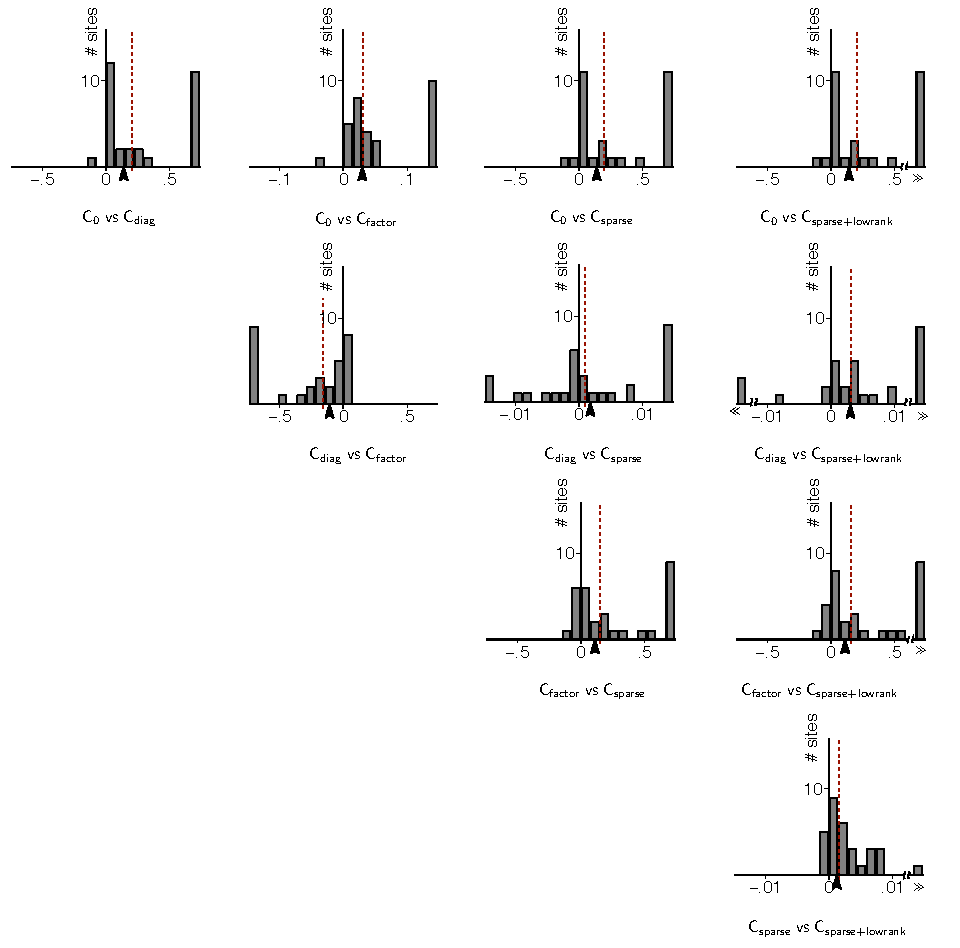
\includegraphics{./figures/Figure-Supp01.pdf}
\end{center}
\caption{{\bf All-to-all performance comparisons of the sample covariance matrix and the four regularized estimators.}
}
\label{supp:01}
\end{figure}
\end{document}
